%preamble
\documentclass[12pt,a4paper]{article}

%###########################################################
%PACOTES DE IDIOMA, ACENTUAÇÃO E FORMATAÇÃO DO DOCUMENTO

\usepackage{indentfirst}
\usepackage[utf8]{inputenc} %Usado para aceitar acentos
\usepackage[T1]{fontenc}
\usepackage[portuguese,brazilian]{babel} %Usado para definir o idioma
%\usepackage[width=0.00cm, left=3.00cm, right=2.00cm, top=2.00cm, bottom=2.00cm]{geometry} %Usado para modificar margens do documento
\usepackage{multicol} %Permite que, quando necessário, utilize duas ou mais colunas em uma parte do texto
\usepackage{color} %Habilita a utilização de cores
\usepackage{lipsum}

%###########################################################
%PACOTES GRAFICOS

\usepackage{graphicx} %Usado para permitir importar imagens
\usepackage[font={small}, labelfont={bf}, margin=1cm]{caption} %Usado para legenda de figuras
\usepackage{float} %para ser usado com o parametro H da caracteristica da figura. Permite inserir a figura forçosamente onde se deseja

%###########################################################
%PACOTES MATEMATICOS

\usepackage{amsmath} %Usado para permitir informações matemáticas
\usepackage{amsfonts} %Usado para permitir informações matemáticas
\usepackage{amssymb} %Usado para permitir informações matemáticas

%###########################################################
%DADOS DO AUTOR E DO DOCUMENTO

\title{Meu documento}
\author{César Felipe Gonçalves da Silva}
\date{19 de dezembro de 2016}

%###########################################################
%INICIO DO CORPO DO TEXTO

%###########################################################
%### Observação: A parte acima vai em todo novo documento###
%###########################################################

\begin{document}

%### INICIO DA SEÇÃO DA PAGINA DE TITULO ###
%### COMENTE TODAS CASO NAO QUEIRA PAGINA DE TITULO ###

%\maketitle

\begin{titlepage}
	\begin{center}
	
	\begin{figure}[!ht]
	\centering
	
\includegraphics[width=0.8\textwidth]{figuras/logo-ufal.png}
	\end{figure}

		%\Huge{Universidade Federal de Alagoas}\\
		\large{Mestrado em Modelagem computacional do conhecimento}\\ 
		\large{Leitura e Escrita de Trabalho Científico}\\ 
		\vspace{15pt}
        \vspace{95pt}
        \textbf{\LARGE{Gerência e configuração de thin switches}}\\
		%\title{{\large{Alejandro - Relatório 01 - Gerência e configuração de thin switches}}}
		\vspace{3,5cm}
	\end{center}
	
	\begin{flushleft}
		\begin{tabbing}
			Aluno: César Felipe Gonçalves da Silva\\
			Professor orientador: Professor Doutor Rafael Amorim Silva \\
			\end{tabbing}
 \end{flushleft}
	\vspace{1cm}
	
	\begin{center}
		\vspace{\fill}
			 Dezembro\\
		 2016
			\end{center}
\end{titlepage}

%### FIM DA SEÇÃO DA PAGINA DE TITULO ###



%### INICIO DA SEÇÃO DA FOLHA DE ROSTO ###
%### COMENTE TODAS CASO NAO QUEIRA FOLHA DE ROSTO ###

\begin{titlepage}
	\begin{center}
	
	\begin{figure}[!ht]
	\centering
	
\includegraphics[width=0.8\textwidth]{figuras/logo-ufal.png}
	\end{figure}

		%\Huge{Universidade Federal de Alagoas}\\
		\large{Mestrado em Modelagem computacional do conhecimento}\\ 
		\large{Leitura e Escrita de Trabalho Científico}\\ 
\vspace{15pt}
        
        \vspace{85pt}
        
		\textbf{\LARGE{Relatório}}
		\title{\large{Título}}
	%	\large{Modelo\\
     %   		Validação do modelo clássico}
			
	\end{center}
\vspace{1,5cm}
	
	\begin{flushright}

   \begin{list}{}{
      \setlength{\leftmargin}{4.5cm}
      \setlength{\rightmargin}{0cm}
      \setlength{\labelwidth}{0pt}
      \setlength{\labelsep}{\leftmargin}}

      \item Primeiro Relatório da Disciplina Leitura e Escrita de Trabalho Científico.

      \begin{list}{}{
      \setlength{\leftmargin}{0cm}
      \setlength{\rightmargin}{0cm}
      \setlength{\labelwidth}{0pt}
      \setlength{\labelsep}{\leftmargin}}

			\item Aluno: César Felipe Gonçalves da Silva\
            \item Professor orientador: Professor Doutor Rafael Amorim Silva\
      		

      \end{list}
   \end{list}
\end{flushright}
\vspace{1cm}
\begin{center}
		\vspace{\fill}
		 Dezembro\\
		 2016
			\end{center}
\end{titlepage}

%### FIM DA SEÇÃO DE FOLHA DE ROSTO ###

%### INICIO DA SEÇÃO DE SUMÁRIO ###
%### COMENTE TODAS CASO NAO QUEIRA SUMÁRIO ###

\newpage
\tableofcontents
\thispagestyle{empty}
\newpage

%### FIM DA SEÇÃO DE SUMÁRIO ###



\begin{abstract}
texto do abstract - texto do abstract - texto do abstract - texto do abstract - texto do abstract - texto do abstract - texto do abstract - texto do abstract - texto do abstract - texto do abstract - texto do abstract - texto do abstract
\end{abstract}

\section{Primeira seção}
Conteudo da primeira seção

\subsection{Subseção da primeira seção}
Conteudo da subseção da primeira seção

\subsubsection{blocos de codigos uteis}
Conteudo da subseção da subseção da primeira seção

\begin{itemize}
\item primeiro item pontificado
\item segundo item pontificado
\end{itemize}

\begin{enumerate}
\item primeiro item enumerado
\item segundo item enumerado
\end{enumerate}

\begin{description}
\item[Primeiro item] primeira descrição
\item[Segundo item] segunda descrição
\end{description}

\begin{equation}
e = mc^2
\end{equation}

\begin{multicols}{2} %o numero "2" indica que esta parte do texto usará 2 colunas
Texto em duas colunas Texto em duas colunas Texto em duas colunas Texto em duas colunas Texto em duas colunas Texto em duas colunas Texto em duas colunas Texto em duas colunas Texto em duas colunas Texto em duas colunas Texto em duas colunas Texto em duas colunas Texto em duas colunas Texto em duas colunas Texto em duas colunas Texto em duas colunas Texto em duas colunas Texto em duas colunas Texto em duas colunas Texto em duas colunas Texto em duas colunas Texto em duas colunas Texto em duas colunas Texto em duas colunas Texto em duas colunas Texto em duas colunas Texto em duas colunas Texto em duas colunas Texto em duas colunas Texto em duas colunas Texto em duas colunas Texto em duas colunas Texto em duas colunas Texto em duas colunas Texto em duas colunas Texto em duas colunas Texto em duas colunas Texto em duas colunas Texto em duas colunas Texto em duas colunas Texto em duas colunas Texto em duas colunas Texto em duas colunas Texto em duas colunas Texto em duas colunas Texto em duas colunas 
\end{multicols}

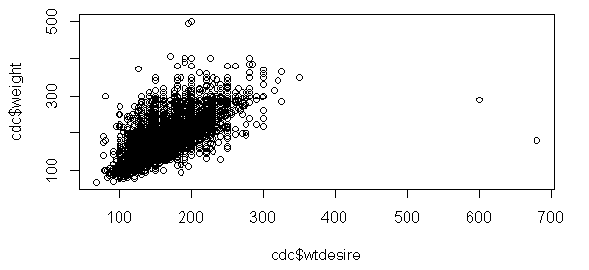
\includegraphics[width=0.8\textwidth]{figuras/q1.PNG} % o Valor 0.8 indica que o grafico terá 80% do tamanho "entre margens" do documento e a parte "figuras/q1.PNG" indica que o arquivo "q1.PNG" esta dentro da pasta "figuras" (que tem que estar dentro da pasta onde se esta salvando o arquivo .TEX)

\begin{center}
\begin{tabular}{l|c|c|r} 
% Observacao 01: "LCCR" indica que a tabela tera 4 colunas, sendo a primeira alinhada à esquerda, as duas seguintes serão centralizadas e a ultima alinhada à direta

%% Observacao 02: Bote | Entre as definições de alinhamento das colunas para informar se haverá linha vertical entre as colunas

%Observação 03: Use \hline ao fim de cada linha para informar se haverá linha horizontal entre as linhas

%Observação 04: Use "&" para separar colunas e use \\ para iniciar nova linha

\hline
Aluno & Nota 1 & Nota 2 & Média \\ \hline
César & 8.0 & 9.0 & 8.5 \\ 
Daiane & 10.0 & 10.0 & 10.0 \\
Maria & 4.0 & 6.0 & 5.0 \\ \hline
& & Media geral & 7.75 \\ \hline

\end{tabular}
\end{center}

\newpage %Use isto sempre que quiser criar uma nova pagina
Aqui vem o conteudo da primeira pagina nova criada

\newpage %Use isto caso queira criar mais uma outr pagina, fora a que ja foi criada acima
Aqui vem o conteudo da segunda pagina nova criada


\end{document}